\documentclass[a4paper,11pt]{article}
\usepackage[utf8]{inputenc}
\usepackage[T1]{fontenc}
\usepackage[english]{babel}
\usepackage{amsmath,amssymb,amsthm,amsopn}
\usepackage{mathrsfs}
\usepackage{graphicx}
\usepackage{tikz}
\usepackage{array}
%\usepackage[top=1cm,bottom=1cm]{geometry}
%\usepackage{listings}
\usepackage{xcolor}
\usepackage{hyperref}
\hypersetup{
    colorlinks=true,
    linkcolor=blue,
    citecolor=red,
}

% Tikz style
\tikzset{round/.style={circle, draw=black, very thick, scale = 0.7}}
\tikzset{arrow/.style={->, >=latex}}
\tikzset{dashed-arrow/.style={->, >=latex, dashed}}

\newtheoremstyle{break}%
{}{}%
{\itshape}{}%
{\bfseries}{}%  % Note that final punctuation is omitted.
{\newline}{}

\newtheoremstyle{sc}%
{}{}%
{}{}%
{\scshape}{}%  % Note that final punctuation is omitted.
{\newline}{}

\theoremstyle{break}
\newtheorem{thm}{Theorem}[section]
\newtheorem{lm}[thm]{Lemma}
\newtheorem{prop}[thm]{Proposition}
\newtheorem{cor}[thm]{Corollary}
\newtheorem{heur}[thm]{Heuristic}

\theoremstyle{sc}
\newtheorem{exo}{Exercise}

\theoremstyle{definition}
\newtheorem{defi}[thm]{Definition}
\newtheorem{ex}[thm]{Example}

\theoremstyle{remark}
\newtheorem{rem}[thm]{Remark}

\DeclareMathOperator{\Ker}{Ker}
\DeclareMathOperator{\Id}{Id}
\DeclareMathOperator{\Img}{Im}
\DeclareMathOperator{\Card}{Card}
\DeclareMathOperator{\Vect}{Vect}
\DeclareMathOperator{\Tr}{Tr}
\DeclareMathOperator{\pgl}{PGL}


% Nouvelles commandes
\newcommand{\ps}[2]{\left\langle#1,#2\right\rangle}
\newcommand{\ent}[2]{[\![#1,#2]\!]}
\newcommand{\diff}{\mathop{}\!\mathrm{d}}
\newcommand{\ie}{\emph{i.e.\ }}
\newcommand{\eg}{\emph{e.g.\ }}
% know what is going on or when I still need to ckeck

% opening
\title{Internship report\\\textbf{Discrete logarithm in finite fields of
small characteristic}}
\author{Édouard \textsc{Rousseau}\\\textit{Supervised by}\\Éric \textsc{Schost} and Luca
\textsc{De Feo}}

\begin{document}

\maketitle
\begin{verbatim}
               _
   _       _ _(_)_     |  A fresh approach to technical computing
  (_)     | (_) (_)    |  Documentation: http://docs.julialang.org
   _ _   _| |_  __ _   |  Type "?help" for help.
  | | | | | | |/ _` |  |
  | | |_| | | | (_| |  |  Version 0.5.1 (2017-03-05 13:25 UTC)
 _/ |\__'_|_|_|\__'_|  |  Official http://julialang.org/ release
|__/                   |  x86_64-pc-linux-gnu

julia> using DlogGF

Welcome to

         8I  ,dPYb,                       
         8I  IP'`Yb                        
         8I  I8  8I                          .oooooo.    oooooooooooo   
         8I  I8  8'                         d8P'  `Y8b   `888'     `8  
   ,gggg,8I  I8 dP    ,ggggg,     ,gggg,gg 888            888         
  dP'  'Y8I  I8dP    dP'  'Y8ggg dP'  'Y8I 888            888oooo8     
 i8'    ,8I  I8P    i8'    ,8I  i8'    ,8I 888     ooooo  888    '     
 d8,   ,d8b,,d8b,_ ,d8,   ,d8'  d8,   ,d8I `88.    .88'   888           
 'Y8888P'`Y88P''Y88P'Y8888P'    'Y8888P'888  `Y8bood8P'   o888o           
                                      ,d8I'                              
                                    ,dP'8I                               
                                   ,8'  8I                               
                                   I8   8I                               
                                   `8, ,8I                               
                                    `Y8P'                             
\end{verbatim}
\clearpage
\begin{abstract}
This internship took place from March to September 2017 in the Symbolic
Computation Group of the University of Waterloo. We studied the recent
breakthroughs in the discrete logarithm world, in the finite field of small characteristic case.
As part of this study, we implemented the encountered algorithms and made them
available as an open-source library written in Julia/Nemo~\cite{Julia, Nemo}.
\end{abstract}

\tableofcontents
\clearpage

\section{Introduction}

With the rise of new technologies and new communication media, the importance of
cryptography has been steadily growing. In 1976, a new era of cryptography was
born, with the invention of \emph{public-key} cryptography by Diffie and
Hellman, in their article ``New Directions in Cryptography''~\cite{DH76}. Today,
cryptography is omnipresent, though mostly invisible to the user. Even if
millions of executions of public-key protocols happen each second, there are only two
main families those protocols are drawn from. Indeed, they are
very often based either on integer factorization (like the well known
and extensively used RSA protocol), or on discrete logarithm. The Discrete
Logarithm Problem (DLP) is fairly easy to state. Let $\mathcal G=\left\langle
g\right\rangle$ be a cyclic group generated by an element
$g$, and denote by $N=|\mathcal G|$ its cardinal. We have the isomorphism:
\[
 \begin{array}{cccc}
   \exp_g: & \mathbb{Z}/N\mathbb{Z} & \to & \mathcal G \\
   & n & \mapsto & g^n,
 \end{array}
\]
and we denote by $\log_g=\exp_g^{-1}$ the inverse isomorphism (sometimes only
denoted by $\log$). In practice, the
\emph{square and multiply} algorithm allows us to compute $g^n=\exp_g(n)$
efficiently, \ie in polynomial time. But, given $y = g^k$, the computation of $k
= \log_g(y)$ is not as easy. This kind of function $f$, where $f$ is easy to
compute but $f^{-1}$ is hard to compute, is called \emph{one-way} function.
It is
typically used in cryptology to make the encryption fast and the deciphering
slow. 

In fact, discrete
logarithms were studied long before their utilization in cryptography. Indeed,
Gauß, in its \emph{Disquisitiones Arithmeticae}, back in 1801, was already
computing discrete logarithms, that he reffered to as \emph{indices}.
Nevertheless, the discrete logarithm really became a practically relevant problem
with the invention of the Diffie-Hellman key exchange protocol~\cite{DH76}. The
security of the protocol originally relied on the hardness of the discrete
logarithm problem in $(\mathbb{Z}/N\mathbb{Z})^\times$. This group is no longer
secure, but other interesting groups can be used, such as the points of an
elliptic curve or the multiplicative group of a finite field. In this
internship, we focused on that last case. Over the years, two
types of algorithms emerged:
\begin{itemize}
  \item the \emph{generic} algorithms, that can be used for any group, with an
    exponential complexity of type $O(\sqrt N)$, where $N=|\mathcal G|$ is the cardinal
    of the group;
  \item the \emph{index calculus} algorithms, that are built on the structure of
    the group considered, and that have very different complexities, depending
    on the kind of group.
\end{itemize}

To express the complexity of an algorithm, one typically uses the notation
\[
  L_N(\alpha, c) = \exp((c+o(1))(\log N)^\alpha(\log\log N)^{1-\alpha})
\]
where $\alpha\in[0, 1]$, $c>0$, and $\log$ represents the natural logarithm. We may
omit the subscript $N$ if there is no ambiguity, or even write
$L(\alpha)$ to indicate $L(\alpha, c)$ for some constant $c>0$, if we do not
want to specify the constant. This notation can be seen as an interpolation
between the polynomial complexity $L(0)=(\log N)^{c+o(1)}$ and the exponential
complexity $L(1)=N^{c+o(1)}$. An algorithm with complexity $L(\alpha)$, for
$0<\alpha<1$, is said to have \emph{sub-exponential} complexity.

When Diffie and Hellman wrote their article in 1976, the known algorithms
had exponential complexities. The first sub-exponential algorithm for the
discrete logarithm in finite fields was analysed
in 1979 by Adleman~\cite{Adleman79}, it has complexity $L(1/2)$. In 1984, 
Coppersmith designed
an algorithm to handle the case of binary fields~\cite{Coppersmith84} with 
complexity $L(1/3)$. Other
algorithms were invented, generalized, or improved, among them the FFS
(Function Field Sieve) and NFS (Number Field Sieve), so that in 2006, every type
of finite field was covered with complexity $L(1/3)$. This complexity remains
the best in medium and large characteristic. In the small
characteristic case, however, there has been a series of dramatic
improvements that leave us with \emph{quasi-polynomial} algorithms. If we denote
by $l$ the bitlength of the finite field in which we work, a quasi-polynomial
complexity is of the form
\[
  l^{O(\log l)}.
\]
This complexity is smaller than $L(\varepsilon)$ for any
$\varepsilon>0$, but larger than the polynomial complexity $L(0)$, so it
is sometimes denoted as $L(o(1))$.

The recent algorithms that achieve quasi-polynomial complexity are index
calculus algorithms, so we introduce this method in
Section~\ref{index-calculus}. We recall the new ideas that led to a new family
of algorithms achieving quasi-polynomial complexiy, the so-called Frobenius representation algorithms, in Section~\ref{quasi-pol}. We study the first quasi-polynomial algorithm, due to
Barbulescu, Gaudry, Joux and Thomé in Section~\ref{bgjt}. In particular we show
how to compute the logarithms of the factor base in this section. We study the
second quasi-polynomial algorithm, due to Granger, Kleinjung and Zumbrägel,
which is more efficient in practice, in Section~\ref{powers-of-2}. Finally, we
give our experimental results in Section~\ref{sec:results}.

\section{The index calculus method}
\label{index-calculus}

Here again, we consider a group $\mathcal G=\left\langle g \right\rangle$, an element
$g^k = h\in \mathcal G$, and we want to compute $k$. The index calculus algorithms always
follow the same pattern:
\begin{enumerate}
  \item[0.] we choose a subset $\mathcal F\subset \mathcal G$ such that $\left\langle
    \mathcal F \right\rangle = \mathcal G$
    (we often have $g\in \mathcal F$), this subset is called the \emph{factor base};
  \item we generate multiplicative relations between the elements of $\mathcal F$, \ie we
    find $f_1, \dots, f_n \in \mathcal F$ and $e_1, \dots, e_n\in \mathbb{Z}$ such that
    $\prod_i f_i^{e_i} = 1$, that is equivalent to the linear equation $\sum_i
    e_i\log_g(f_i) = 0$;
  \item we solve the linear system with unknowns $\log_g(f_i)$ arising from step
    1 to obtain $\log(f)$ for all $f\in \mathcal F$;
  \item we find a multiplicative relation between $h$ and elements of $\mathcal F$, or
    equivalently, we express $\log_g h = k$ as a linear combination of the
  $\log_g(f_i)$.
\end{enumerate}
As a first example, we introduce Adleman's algorithm. We let $\mathcal
G=\mathbb{F}_p^\times$ be the multiplicative group of a prime field
$\mathbb{F}_p=\mathbb{Z}/p\mathbb{Z}$, and we let our factor base be 
\[
  \mathcal F =\left\{ f\;|\;f\leq B, f\text{ prime} \right\}
\]
where $B\in \mathbb{N}$ is an integer that has yet to be determined, and where
we make the abuse of denoting by $f$ both the integer
$f\in\mathbb{N}$ and its class $\bar f\in\mathbb{F}_p$. We assume that
$g\in\mathcal F$, otherwise we add $g$ to $\mathcal F$. In order to generate
multiplicative relations, we take a random $e\in\mathbb{Z}/(p-1)\mathbb{Z}$ and
we compute $g^e$, we say that $e$ yields a relation if the lift
$g^e\in\mathbb{N}$ is $B$-smooth, \ie if $g^e$ has only prime divisors $\leq B$.
In that case we have a relation 
\[ 
  g^e \equiv \prod_{f\in \mathcal F}f^{e_f} \mod p
\]
in the integers, that becomes 
\[ 
  g^e = \prod_{f\in \mathcal F}f^{e_f}
\]
in $\mathbb{F}_p$ (with the same abuse of notation), and where the exponents are
just some integers $e_f\in\mathbb{N}$. In terms of the logarithms, we write this
relation
\[
  e = \sum_{f\in\mathcal F} e_f\log f.
\]
Once we have enough relations, meaning more than $|\mathcal F|$, we are able to
recover the unknowns $\log f$ using classic linear algebra algorithms. Note that
the system is usually sparse, since the relations hardly contain all the
elements $f\in\mathcal F$. If the target element is some $h\in\mathcal G$, we
proceed in the same way to recover $\log h$. We take some
$e\in\mathbb{Z}/(p-1)\mathbb{Z}$ at random and compute $hg^e$. Once again, if
the lift of $hg^e$ is $B$-smooth, we have an equation of type
\[
  \log h + e = \sum_{f\in\mathcal F}h_f\log f
\]
where the $h_f\in\mathbb{N}$ are integers and all the $\log f$ are now known, so
we are able to recover the logarithm of $h$. The larger $B$ is, the easier it is
to obtain multiplicative relations. But at the same time, the size of $\mathcal
F$ will also become larger and we will need more multiplicative relations to
compute all the unknowns $\log f$. Adleman~\cite{Adleman79} showed that with a suitable choice of
$B$, this algorithms has a $L(1/2)$ complexity.

Even if the pattern is almost identical in every index calculus algorithm, there
are a lot of available strategies to generate multiplicative relations and
express the target element as a combination of elements in the factor base. This
has led to a rich variety of algorithms, among them are the quasi-polynomial
algorithms. We introduce them briefly in the next section.

\section{Quasi-polynomial algorithms}
\label{quasi-pol}

There are two quasi-polynomial algorithms, the BGJT algorithm~\cite{BGJT13} and
the powers-of-2 algorithm~\cite{GKZ14}, they are respectively studied in
Section~\ref{bgjt} and~\ref{powers-of-2}. They were published almost at the
same time, in 2013 and 2014, and are independant. 
The main ideas for those algorithms were already present in a
previous work of Joux~\cite{Joux13}, published earlier in 2013 and leading to
an algorithm with complexity $L(1/4 + o(1))$. Before giving those ideas, we
recall the general setup in which we perform the algorithms.

\subsection{Setup}
\label{general-setup}

Let $\mathcal G = (\mathbb{F}_{q^n})^\times$ be the multiplicative group of a finite
field of small characteristic $\mathbb{F}_{q^n}$, where $q=p^l$ is a prime
power. By
\emph{small characteristic} we mean that $q$ must be a polynomial in the size of
the field $q^n$, \ie $q = L_{q^n}(0)$. In other documents, the term ``small
characteristic'' may indicate that $q = L_{q^n}(\alpha)$ for
$\alpha<\frac{1}{3}$, but this assumption would break the quasi-polynomial
nature of these algorithms. We represent elements of
$\mathbb{F}_{q^n}$ by polynomials over $\mathbb{F}_{q}$ of degree less than
$n$. The factor base $\mathcal F\subset\mathcal G$ will contain elements
represented by irreducible polynomials up to a certain degree, depending on the
algorithm. We have not made
precise what polynomial $P$ we use to represent
$\mathbb{F}_{q^n}\cong\mathbb{F}_{q}[X]/(P)$, but this is done
in Section~\ref{ideas}. Again, we will make a notation abuse: if we have
$Q\in \mathbb{F}_{q}[X]$, we will still write $Q$ for the class $\bar Q\in
\mathbb{F}_{q}[X]/(P)$. Conversely, if we have an element $Q\in
\mathbb{F}_{q^{n}}$, we
will also denote by $Q$ the polynomial in $\mathbb{F}_{q}[X]$ representing the
element.

\subsection{Background ideas}
\label{ideas}

In the case of $\mathbb{Z}/p\mathbb{Z}$, we used the decomposition of the
integers into prime factors to generate multiplicative relations. The situation
here is analogous: we decompose some polynomials into irreducible polynomials of
lower degree to get relations. Before going into details, we list three ideas
(first stated in~\cite{Joux13}) used in the algorithms.

\paragraph{Idea 1: homographies.} Given a polynomial $Q$ that factors \emph{nicely}
(and thus is susceptible to give \emph{nice} relations), we can produce a lot of other
polynomials using changes of variables induced by homographies:
\[
  X\to\frac{aX+b}{cX+d}.
\]
We see that $Q(\frac{aX+b}{cX+d})$ is not a polynomial, so by change of variable
using homographies, we mean homogeneous evaluation at $\frac{aX+b}{cX+d}$,
that is, the polynomial:
\[
  Q_{abcd}(X) = (cX+d)^{\deg Q}Q\left(\frac{aX+b}{cX+d} \right).
\]
If we have the decomposition $Q=\gamma\prod_j Q_j$, with $\gamma$ a constant and
$Q_j$ irreducible monic polynomials, then we also have
\[
  Q_{abcd}(X) = \gamma\prod_j (cX+d)^{\deg Q_j}Q_j(\frac{aX+b}{cX+d})
\]
but the new factors in this decomposition are not necessary irreducible, not
necessary monic and may even have a lower degree than the original $Q_j$.

\paragraph{Idea 2: systematic polynomial splitting.} The second idea is to use
the polynomial $X^q-X$ because we already know that it factors into linear
polynomials over $\mathbb{F}_q$. Thus, instead of looking for a random candidate to
apply the first idea, we always use $X^q-X$.

\paragraph{Idea 3: defining polynomial.} We want to take advantage of the liberty that we
have for the irreducible polynomial $P$ defining
$\mathbb{F}_{q^{n}}=\mathbb{F}_{q}[X]/(P)$. In fact, by using the ideas $1$ and
$2$, we somehow favor the term $X^q$ and spread it in our equations. That is why
we make a choice of $P$ that transforms $X^q$ into something simpler. To do
that, we ask $P$ to be an irreducible factor of degree $n$ of
$h_1(X)X^q-h_0(X)$,
where $h_0, h_1\in\mathbb{F}_{q}[X]$ are polynomials of low degree $\delta$
(in practice, we take $\delta\leq2$). If we
denote by $x$ the class of $X$ in $\mathbb{F}_{q^{n}}$, we have
\[
  x^q=\frac{h_0(x)}{h_1(x)}.
\]
Since this construction requires a simple expression of the map $x\mapsto x^q$, it
is called \emph{Frobenius representation}. It is not known if it is always
possible to find suitable polynomials $h_0, h_1$, the fact that every finite
field can be represented that way is an \emph{heuristic}. This construction
might be impossible simply because $n > q+\delta$, but in fact, we can always
assume that we have $n\leq q+\delta$ by embedding our field
$\mathbb{F}_{q^n}$ into a bigger
one. Let us start again from scratch: let $\mathbb{F}_{p^n}$ be the finite field
in which we want to solve the DLP and let $q=p^l$ be the smallest power of $p$ such
that $q\geq n$. Then we embed $\mathbb{F}_{p^n}$ into
$\mathbb{F}_{p^{ln}}=\mathbb{F}_{q^n}$ and we actually solve the DLP in $\mathbb{F}_{q^n}$. From now
on, we will always assume that $\mathbb{F}_{q^n}$ has been constructed that way,
so that there is no obstruction to the Frobenius representation.

These ideas are used both to find relations between the elements in the factor
base and to express a target element as a combination of elements in the base.
In general, this last operation cannot be done in one single step. Instead, the
target element will be expressed as ``simpler'' elements, \ie elements
represented by polynomials with lower degrees. This strategy is applied
recursively until all the elements are in the factor base $\mathcal F$, this
whole operation is called the \emph{descent}. We give more details in next
section.

\section{The BGJT algorithm}
\label{bgjt}

The BGJT algorithm gets its name from its authors: Barbulescu, Gaudry, Joux and
Thomé. It was first published in 2013~\cite{BGJT13} and it is the first
(heuristic) quasi-polynomial algorithm. The setup is slightly different from the
general one given in Section~\ref{general-setup}, it is the same as the original
one given in the article.

\subsection{Setup of the BGJT algorithm}

Let $\mathcal G = (\mathbb{F}_{q^n})^\times$ the multiplicative group of a finite
field of small characteristic $\mathbb{F}_{q^n}$, where $q=p^l$ is a prime
power. We also assume that there is a ``medium subfield'' in
$\mathbb{F}_{q^n}$, \ie a field of size $\mathbb{F}_{q^2}$. In other words, we
ask that $n = 2m$ for some $m>0$. If this is not the case, we first embed our
field $\mathbb{F}_{q^n}$ in a larger field. Thus, we represent elements of
$\mathbb{F}_{q^n} = \mathbb{F}_{q^{2m}} = \mathbb{F}_{q^2}[X]/(P)$ by
polynomials over $\mathbb{F}_{q^2}$ of degree less than
$m$. As described in Section~\ref{ideas}, the polynomial $P$ is an irreducible
polynomial of degree $m$ dividing $h_1(X)X^q-h_0(X)$, where $h_0,
h_1\in\mathbb{F}_{q^2}[X]$ are polynomials of small degree. Heuristically, it
seems that taking polynomials of degree $2$ is sufficient. Our factor base
$\mathcal F\subset\mathcal G$ will be the set of elements represented by degree
one polynomials. Using the relation $X^q=\frac{h_0(X)}{h_1(X)}$, a power of
$h_1$ appears in all equations, so we also add $h_1$ to the factor base
$\mathcal F$. When we target an element $h\in\mathbb{F}_{q^{2m}}$, we implicitly
assume that a basis for the discrete logarithm has been chosen and that $h$
belongs to a subgroup of $\mathcal G$ whose order has no small irreducible
factor. This assumption is possible thanks to the use of the Pohlig-Hellman
algorithm~\cite{PH78}.

\subsection{Main results and complexity}

Now that we have the setup for the algorithm, we can state the main results and
explain how to use them to recover the discrete logarithm of an element in
$\mathbb{F}_{q^{2m}}$. The following results is used to express an element as
``simpler elements''.

\begin{prop}
  \label{prop:bgjt}
  Let $K = \mathbb{F}_{q^{2m}}$ be a finite field with the structure discussed below.
  There exists a heuristic algorithm whose complexity is polynomial in $q$ and
  $m$ and which can be used for the following task. Given an element of $K$ represented by a polynomial
  $Q\in\mathbb{F}_{q^2}[X]$ with $2\leq \deg Q \leq m-1$, the algorithm
  returns an expression of $\log Q$ as a linear combination of at most
  $O(q^2m)$ logarithms $\log Q_j$ with $\deg Q_j\leq
  \lceil\frac{1}{2}\deg Q\rceil$ and of $\log h_1$.
\end{prop}

In order to compute the logarithms of the linear elements and $h1$, \ie the
factor base, we use this second proposition.

\begin{prop}
  \label{prop:bgjt2}
  Let $K = \mathbb{F}_{q^{2m}}$ be a finite field with the structure discussed below.
  There exists a heuristic algorithm whose complexity is polynomial in $q$ and
  $m$ and that returns the logarithm of $h_1$ and of the logarithms of
  all the elements of $K$ of the form $X+a$ for $a\in\mathbb{F}_{q^2}$.
\end{prop}

Before explaining how to perform the algorithms,
we show how to use them to recover the discrete logarithm of an element, and we
discuss the complexity of such a process. Let $h\in\mathbb{F}_{q^{2m}}$ be a
target element, we denote by $Q\in\mathbb{F}_{q^2}[X]$ the polynomial
representing $h$, and we assume that $2\leq \deg Q\leq m-1$, otherwise $h$ is
already in the factor base $\mathcal F$. We start by applying
Proposition~\ref{prop:bgjt} to $Q$, so we obtain a relation of the form
\[
  \log Q = q_0\log h_1 + \sum_j q_j\log Q_j
\]
where the sum has at most $O(q^2m)$ terms and where $\deg
Q_j\leq\lceil\frac{1}{2}\deg Q\rceil$ for all $j$. We then apply
Proposition~\ref{prop:bgjt}
recursively to the $Q_j$'s, creating a descent process in which the logarithm of
each element is expressed as a linear combination of the logarithms of other
elements with degrees twice as small (rounded up). By Proposition~\ref{prop:bgjt}, the
arity of the descent tree is in $O(q^2m)$. At the end of the process, the
logarithm of $Q$ is expressed as a linear combination of linear polynomials and
of $h_1$. These are the elements of the factor base, and we can find their
logarithm thanks to Proposition~\ref{prop:bgjt2}.

The cost of each use of Proposition~\ref{prop:bgjt} is bounded by a polynomial in $q$ and
$k$, and each node of the descent tree corresponds to one application of the
proposition. The complexity of the descent is therefore bouned by the number of
nodes times a polynomial in $q$ and $k$. Since the degree of the polynomials
involved is divided by two during each step, the depth of the tree is
$O(\log m)$. The number of nodes in a tree is bounded by its arity raised to the power
of its depth, so the number of nodes is bounded by $(q^2m)^{O(\log m)}$. Since
any polynomial is absorbed in the $O()$ notation in the exponent, we can
conclude that the descent has a complexity bounded by
\[
  \max(q, m)^{O(\log m)}.
\]
In the original article~\cite{BGJT13}, the authors discuss the consequences of
such a result for various ranges of parameters. In our case, where we assume
that $q$ is polynomial in the size of the input field $l=\log|\mathbb{F}_{q^{2m}}|$ and
$q\geq m$, we can write the complexity
\[
  l^{O(\log l)}.
\]
Therefore, we have the claimed quasi-polynomial complexity. Note that if we had
$q = L_{q^{2m}}(\alpha)$ with some value $\alpha<\frac{1}{3}$, the complexity of the BGJT
algorithm would be in
$L_{q^{2m}}(\alpha+o(1))$, so it would no longer be quasi-polynomial. Nevertheless, even if
less impressive than quasi-polynomial complexity, $L_{q^{2m}}(\alpha+o(1))$ is
still better than previously known algorithms for large families
of finite
fields. Now that we have a global view of how to compute a discrete logarithm,
we explain the algorithms the propositions refer to.

\subsection{Proof of Proposition~\ref{prop:bgjt} and Proposition~\ref{prop:bgjt2}}

We start with Proposition~\ref{prop:bgjt}, but as we will see, the method
used in the second proposition is essentially the same. Let $Q$ be the element to
be eliminated, \ie to be expressed as ``simpler'' elements, 
the strategy is to find relations involving $Q$ and its
translates by a constant $Q-\xi$, where $\xi\in\mathbb{F}_{q^2}$. We use a
projective version of the
\emph{systematic equation}:
\[
  X^q - X = \prod_{u\in\mathbb{F}_q} X-u 
\]
obtained via homogenization that we write as a product on the projective
line $\mathbb{P}_1(\mathbb{F}_q)$:
  \begin{equation} 
  X^qY-XY^q = \prod_{\alpha\in\mathbb{P}_1(\mathbb{F}_q)} X - \alpha Y.
    \label{proj-eq}
  \end{equation}
In this slightly abusive notation, when $\alpha=(u:1)$ is not the point at
infinity, the expression $X-\alpha Y$ simply means $X-uY$, whereas when
$\alpha=(1:0)$ is the point at infinity, the expression $X-\alpha Y$ means $Y$.

To make the translates appear, we will use homographies, denoted by
matrices $m=\begin{pmatrix} a&b\\c&d\end{pmatrix}$, on
Equation~\eqref{proj-eq}, where $a, b, c, d\in\mathbb{F}_{q^2}$. With each element $m$, we associate the equation
$(E_m)$ by substituting $X$ by $aQ+b$ and $Y$ by $cQ+d$.
\begin{align}
  (aQ+b)^q(cQ+d)-(aQ+b)(cQ+d)^q &=
  \prod_{\alpha\in\mathbb{P}_1(\mathbb{F}_q)}(aQ+b)-\alpha(cQ+d)\nonumber\\
  &= \prod_{\alpha\in\mathbb{P}_1(\mathbb{F}_q)}(a-\alpha c)Q+b-\alpha
  d\nonumber\\
  \label{eqn:Em}
  \tag{$E_m$}
  &=
  \lambda\prod_{\alpha\in\mathbb{P}_1(\mathbb{F}_q)}Q-m^{-1}\cdot\alpha.
\end{align}

Again, in the products of the two first lines, some care has to be taken about
the meaning of the terms, but the explicit meaning
follows directly from the explanations given
above. In the last line, that gives our Equation~\eqref{eqn:Em}. The notation
$Q-m^{-1}\cdot\alpha$ means $Q-u$ if $m^{-1}\cdot\alpha=(u:1)$; it
means $1$ if $m^{-1}\cdot\alpha=\infty=(1:0)$.
Finally, $\lambda\in\mathbb{F}_{q^2}$ is the constant such that the equality
holds.

In the end, we just reorganized the terms by factoring the constants multiplying $Q$.
Note that one of the constants could be zero and the term $Q$ could then vanish,
this is happening when $m^{-1}\cdot\alpha=\infty$. Therefore, the right hand of
Equation~\eqref{eqn:Em} is, up to a multiplicative constant, a product of $q+1$ or $q$
translates of $Q$.

At this point, one may wonder what we mean by $m^{-1}$, since we
did not specify anything about $m$. In fact, we have some constraints on this
matrix. If $m$ is not invertible, we have only one translate appearing in the
right hand side, leading to a trivial relation that we will not exploit. If the
constants $a, b, c, d$ are all in $\mathbb{F}_q$, the relation generated is, up
to a constant in $\mathbb{F}_q$, always the same, so we consider this case
trivial too. Finally, we can see that multiplying all the coefficients by a
non-zero constant will lead to the same relation, up to a constant, so we
consider this trivial again. We consider that the relations are the same when
they differ by a constant because the logarithms of the constants are easy to
find: since $\mathbb{F}_{q^2}$ contains $q^2$ elements, and since $q$ is a
polynomial in the size of the input, we can find the logarithms of all the
constants in polynomial time by computing $\zeta^j$ for $1\leq j \leq q^2-1$ and
$\zeta$ a generator of $\mathbb{F}_{q^2}^\times$. All that being said, we conclude that we have to take
$m$ in the set of cosets:
\[
  \mathcal P_q = \pgl_2(\mathbb{F}_{q^2})/\pgl_2(\mathbb{F}_q).
\]
Note that in general $\pgl_2(\mathbb{F}_q)$ is not a normal subgroup of
$\pgl_2(\mathbb{F}_{q^2})$, therefore $\mathcal P_q$ is not a quotient group,
but only a set of cosets. We do not have a nice way of iterating
through its elements perfectly, \ie visiting each element only once and in
$|\mathcal P_q|$ steps, but an efficient algorithm has been written
in~\cite{ZC15}. It is a general result that
$|\pgl_2(\mathbb{F}_{q^j})|=q^{3j}-q^j$, so the number of elements in the set of
cosets $\mathcal P_q$ is $|\mathcal P_q| = (q^6-q^2)/(q^3-q)=q^3+q$.

Now, let us go back to our Equation~\eqref{eqn:Em}. On the left side of the equation, we have a polynomial of high degree that seems
hard to exploit. But recall that, with the choice of defining polynomial for our
field $\mathbb{F}_{q^{2m}}$, we have $X^q \equiv \frac{h_0(X)}{h_1(X)}$. This will
be used to lower the degree on the left hand side. Let us denote by $\tilde a$
the element $a^q$ for any $a\in\mathbb{F}_q^2$. Similarly, we denote by
$\widetilde Q$ the polynomial $Q$ with all its coefficients raised to the power
$q$. We can now write the left hand of Equation~\eqref{eqn:Em}
\[
  (\tilde a \widetilde Q (X^q)+\tilde b)(cQ(X)+d)-(aQ(X)+b)(\tilde c\widetilde
  Q(X^q)+\tilde d),
\]
and using the defining polynomial for $\mathbb{F}_{q^{2m}}$, the left hand side of
Equation~\eqref{eqn:Em} is congruent to the following.
\begin{equation}
  \tag{$\mathcal L_m$}
  \left(\tilde a \widetilde Q \left(\frac{h_0(X)}{h_1(X)}\right)+\tilde
  b\right)(cQ(X)+d)-(aQ(X)+b)\left(\tilde c\widetilde
  Q\left(\frac{h_0(X)}{h_1(X)}\right)+\tilde d\right)
  \label{eqn:Lm}
\end{equation}
The denominator of~\eqref{eqn:Lm} is a power of $h_1$, whose logarithm is supposed
to be known, and its numerator has a much smaller degree than the original one
in~\eqref{eqn:Em}. Indeed, the numerator of~\eqref{eqn:Lm} has degree at most
$(1+\delta)\deg Q$, where $\delta=\max(\deg h_0, \deg h_1)$ (we can assume
$\delta=2$ in practice), whereas the original degree in~\eqref{eqn:Em} is at
most $(1+q)\deg Q$ (and we can have $q = 3^5 = 243$ in practice,
see~\cite{Adj16} for an example).

But we did not explain why we want small degree polynomials so much in our
equations. The answer is probabilistic: it is more likely that a polynomial
has only irreducible factors of small degree if it has small degree itself. We
say that a polynomial $Q$ is $D$-smooth is it has only irreducible factors of
degree smaller that $D$. Hence, the probability that $Q$ is $D$-smooth, for a
fixed $D$, increases when the degree of $Q$ decreases. In our case, we are
interested in $\lceil\frac{1}{2}\deg Q\rceil$-smooth polynomials. We say that
$m\in\mathcal P_q$ yields a relation if the numerator of~\eqref{eqn:Lm} is
$\lceil\frac{1}{2}\deg Q\rceil$-smooth. We will keep only the equations such
that $m$ yields a relation, and we will remember the translates involved in
the right hand side of Equation~\eqref{eqn:Em}.

To any $m\in\mathcal P_q$, we associate a row vector $v(m)$ of size $q^2+1$
indexed by $\xi\in\mathbb{P}_1(\mathbb{F}_{q^2})$. Each coordinate is either $1$
or $0$, depending on if the term $Q-u$ for $\xi=(u:1)$ appears or not in the
right hand side of Equation~\eqref{eqn:Em}. If there
are only $q$ terms in the product, we put $1$ in position $\xi=\infty$. Hence, we
always have exactly $q+1$ non-zero coordinates in $v(m)$. Equivalently, we can
write
\[
  v(m)_{\xi\in\mathbb{P}_1(\mathbb{F}_q^2)}=\begin{cases} 1\text{ if
    }\xi=m^{-1}\cdot\alpha\text{ with }\alpha\in\mathbb{P}_1(\mathbb{F}_q) \\ 0\text{
    otherwise} \end{cases}.
\]
We construct a matrix $H(Q)$ whose rows are the $v(m)$ for which $m$ yields a
relation, taking at most one matrix $m$ in each coset. We see that $H(Q)$ has
$q^2+1$ columns but the number of rows depends on $Q$. In fact, we are able to
bound from below the probability that $m$ yields a relation by a constant $\kappa$
(see~\cite{BGJT13} for details),
therefore, since $m\in\mathcal P_q$ and $|\mathcal P_q|=q^3+q$, the number of
rows in $H(Q)$ is $\Theta(q^3)$. In order to finish the proof of
Proposition~\ref{prop:bgjt}, we need the following heuristic.
\begin{heur}
  \label{heur:full-rank}
  For any polynomial $Q\in\mathbb{F}_{q^{2}}[X]$, the set of rows $v(m)$ for
  cosets $m\in\mathcal P_q$ that yield a relation forms a matrix $H(Q)$ of
  full rank $q^2+1$.
\end{heur}

We implicitly ask for $q$ to be large enough for $\Theta(q^3)$ to be larger than
$q^2+1$, otherwise the heuristic cannot hold. In other words, we ask the matrix
$H(Q)$ to be sufficiently random to be invertible.
Proposition~\ref{prop:bgjt} follows from linear algebra on $H(Q)$. Since the
matrix has full rank, there is a linear combination of the rows leading to the
vector $(1, 0, \dots, 0)$. We can also assume that the first element in our
iteration of $\mathbb{P}_1(\mathbb{F}_{q^2})$ is $\xi=(0:1)$, such that a $1$ in
the first position corresponds to the term $Q$ in the right hand side of
Equation~\eqref{eqn:Em}. Thus, saying that $(1, 0, \dots, 0)$ can be written as
a linear combination of the rows of $H(Q)$ is equivalent to saying that the
polynomial $Q$ can be written as a product of the right hand side of those
Equations~\eqref{eqn:Em} for which $m$ yields a relation. On the left hand side
of this combination, we obtain a product of $\lceil\frac{1}{2}\deg Q\rceil$-smooth
polynomials, which is thus $\lceil\frac{1}{2}\deg Q\rceil$-smooth too. In the end, we
have expressed $\log Q$ as a linear combination of $\log Q_i$ where the $Q_i$
are the irreducible polynomials occuring in the left hand side. Since there are
$O(q^2)$ columns in $H(Q)$, the elimination process involves at most
$O(q^2)$ rows. Each row corresponds to an Equation~\eqref{eqn:Em} whose left
hand side is congruent to~\eqref{eqn:Lm}, and the degree of the numerator
of~\eqref{eqn:Lm} is $(1+\delta)\deg Q$. In the end, $Q$ is expressed as a product
of $O(q^2\deg Q)$ polynomials of degree less that $\lceil\frac{1}{2}\deg
Q\rceil$. The polynomial $h_1$ also appears as the denominator
of~\eqref{eqn:Lm}, but this is not an issue since its logarithm is known. In
this process, we perform some polynomial manipulations and smoothness tests to
know whether $m\in\mathcal P_q$ yields a relation. All these manipulations can
be done in polynomial time in $q$ and $\deg Q\leq m$. The linear algebra part,
performed on a matrix with $q^2+1$ columns, has a cost of $O(q^{2\omega})$,
using asymptotically fast matrix multiplication, or $O(q^5)$ using sparse
matrix techniques (remember we have only $q+1$ non-zero coefficients out of
$q^2+1$). Therefore, we have an algorithm with polynomial time in $q$ and $m$, as
claimed, and Proposition~\ref{prop:bgjt} is proven.

In order to prove Proposition~\ref{prop:bgjt2}, we use the same process with $Q$ replaced by the
polynomial $X$. In this particular case, the right hand side of
Equation~\eqref{eqn:Em} involves only linear polynomials, and the condition
``$m\in\mathcal P_q$ yields a relation'' means that the numerator
of~\eqref{eqn:Lm} factors into linear polynomials. Thus, the generated relations
involve only linear polynomials and $h_1$. That gives a us a linear system whose
unknowns are the $\log X+\xi$ for $\xi\in\mathbb{F}_{q^2}$ and $\log h_1$. We
cannot rely on Heuristic~\ref{heur:full-rank} to know whether this system has
solutions or not, so we need to state another similar heuristic. In practice, we find that the
matrix associated with the system has a kernel of dimension $1$, that is the
best we can hope for because a dimension of $0$ would mean that the only solution is
$\log (X+\xi)=0=\log h_1$ for all $\xi\in\mathbb{F}_{q^2}$ and a dimension larger
than $2$ would mean too many solutions. If we choose the basis of the logarithm
to be a linear element $X+\xi_0$, we are able to recover all the logarithms by
chosing the only solution such that $\log (X+\xi_0)=1$. This concludes the proof
of Proposition~\ref{prop:bgjt} and Proposition~\ref{prop:bgjt2}.

\subsection{Some concluding remarks}

There are $3$ kinds of heuristics used in this algorithms.
\begin{itemize}
  \item The existence of suitable polynomials $h_0$ and $h_1$, which give the
    structure needed to perform the degree reduction in the left hand side
    of~\eqref{eqn:Em} and obtain~\eqref{eqn:Lm}.
  \item Heuristic~\ref{heur:full-rank} and its equivalent in the case
    $Q(X) = X$, needed for the linear algebra step.
  \item Finally, the analysis leading to the bound on the probability that
    $m\in\mathcal P_q$ yields a relation is based on the assumption that the
    numerator of~\eqref{eqn:Lm} has the same probability to be
    $\lceil\frac{1}{2}\deg Q\rceil$-smooth as a random polynomial of the same
    degree.
\end{itemize}
Supporting arguments and experimental results are given in~\cite{BGJT13}. 
Another important fact is that the logarithm of some polynomials cannot
be computed by that process. They are called \emph{problematic polynomials} and
a result is given in~\cite{BGJT13} to overcome this issue without changing the
quasi-polynomial nature of the algorithm. It happens when the polynomial to be
eliminated $Q\neq P$, where $P$ is the defining polynomial of
$\mathbb{F}_{q^{2m}}$, divides the polynomial $h_1(X)X^q-h_0(X)$. In that case,
$Q$ also divides the numerator of~\eqref{eqn:Lm}, making it impossible to link
the logarithm of $Q$ with smaller degree polynomials, or preventing 
Proposition~\ref{prop:bgjt2} to succeed if $Q$ is a linear polynomial.

The main obstacle preventing this algorithm to be very efficient in practice, in
spite of its quasi-polynomial complexity, is the $O(q^2\deg Q)$ arity  of the
descent tree. In the powers-of-2 algorithm, studied in
Section~\ref{powers-of-2}, the arity is smaller and one heuristic is not needed
anymore, making one step towards a heuristic-free algorithm.

\section{The powers-of-2 algorithm}
\label{powers-of-2}

The algorithm gets its name from its design, particularly suited to target
elements with a degree of the form $2^j$. It was written in 2014 by Granger,
Kleinjung and Zumbrägel. Like the BGJT algorithm, it is based on a heuristic
Frobenius representation and on the other ideas of Section~\ref{ideas}.
The setup in which we present the algorithm is slightly different from
the original, thanks to the work of Joux and Pierrot in \cite{JP14}. Indeed,
they remarked that working with polynomials of degree up to $d$ over $\mathbb{F}_q$ is
essentially equivalent to working with linear polynomials over $\mathbb{F}_{q^d}$. Thus,
instead of working with a factor base composed of linear polynomials over
$\mathbb{F}_{q^d}$ (with $d$ usually between $2$ and $4$), we work with a
factor base composed of irreducible polynomials up to degree $d$. Joux and Pierrot
precisely give a way to compute such a factor base in~\cite{JP14}, that is based
on the technique used in the BGJT algorithm~\cite{Joux13, BGJT13} and has a
complexity of $O(q^6)$. Since we work in the case where $q$ is polynomial in the
bitsize of the input field, this precomputation time is polynomial.

\subsection{Setup of the algorithm}

Let $\mathcal G = (\mathbb{F}_{q^n})^\times$ be the multiplicative group of a finite
field of small characteristic $\mathbb{F}_{q^n}$, where $q=p^l$ is a prime
power, and we represent elements of $\mathbb{F}_{q^n}$ by polynomials over
$\mathbb{F}_q$ of degree less than $n$. More
precisely, we consider the field $\mathbb{F}_{q^n}\cong \mathbb{F}_{q}[X]/(P)$
where $P\in \mathbb{F}_{q}[X]$ is an irreducible polynomial of degree $n$ over
$\mathbb{F}_{q}$ dividing $h_1X^q-h_0$, and $h_0, h_1\in \mathbb{F}_q[X]$ are
polynomials of degree at most $2$ over $\mathbb{F}_q$. Different options are
available to choose $h_0$ and $h_1$, and the respective results are 
discussed in~\cite{JP14}. The existence of such parameters $h_0$ and $h_1$ is,
again, heuristic and critical for the algorithm.

We set the factor base $\mathcal F$ to be composed of all the
elements of $\mathcal G$ represented by an irreducible polynomial of degree at
most $4$. We assume that we know the logarithm of each element in
$\mathcal F$. In other words, we assume that the steps $1$ and $2$ of the index
calculus method have already been performed. This can be done by using the BGJT-like
techniques in the paper of Joux and Pierrot~\cite{JP14}. As we already pointed
out in a discussion above, in the original article
the authors proposed to apply 
Proposition~\ref{prop:bgjt2} to the field $\mathbb{F}_{q^4}$. The only remaining
step is then $3$, where we express the logarithm of an element in $\mathcal G$
as the linear combination of the logarithms of elements in $\mathcal F$. In
order to perform that step, we use a descent strategy, like in the BGJT
algorithm. We express the logarithm of the element that we want
to study, denoted by $Q\in\mathcal G$, as a linear combination of 
$q+2$ ``simpler'' elements $Q_j$, \ie elements represented by polynomials of degree twice
as small. Proceeding recursively, we are able to express $\log Q$ as a
linear combination of elements of degree at most $4$, \ie elements in $\mathcal
F$. Before explaining the descent, we have to introduce its building block, the
\emph{on-the-fly} elimination. Unlike the building block of the BGJT algorithm,
namely Proposition~\ref{prop:bgjt}, there is no linear algebra in that step.
\subsection{On-the-fly degree $2$ elimination}
\label{subsec:on-the-fly}

The crucial part of the descent is called the \emph{on-the-fly}
elimination. It allows one to express a degree $2$ polynomial
$Q\in\mathbb{F}_{q^m}[X]$ over $\mathbb{F}_{q^m}$ as a product of degree $1$ 
polynomials over $\mathbb{F}_{q^m}$. The name ``on the fly'' is due to the fact
that no relation gathering or linear algebra is performed during this
elimination. At the core of this elimination we also use the fact that 
polynomials of the form $\mathcal P_B = X^{q+1}-BX+B$ split completely over $\mathbb{F}_{q^m}$ (\ie they are a
product of polynomials of degree $1$ over $\mathbb{F}_{q^m}$) very often. We
denote by
$\mathcal B$ the set of elements $B\in \mathbb{F}_{q^m}$ such that $\mathcal
P_B$ splits completely. In~\cite{Bluher04}, the roots and the splitting field of
$\mathcal P_B$ are studied and it is shown that the cardinality of $\mathcal B$
is approximately $q^{m-3}$.\footnote{$|\mathcal B| =
  \begin{cases}(q^{m-1}-1)/(q^2-1)\text{ if }m\text{ is odd}\\
  (q^{m-1}-q)/(q^2-1)\text{ if }m\text{ is even}\end{cases}$} Thus, if $B\in \mathcal B$,
$a,b,c\in\mathbb{F}_{q^m}$ such that $c\neq ab$, $a^q\neq b$ and
$B=\frac{(b-a^q)^{q+1}}{(c-ab)^q}$, we see by the change of variable
$X\to\frac{ab-c}{b-a^q}X-a$ in $X^{q+1}+aX^q+bX+c$ that the polynomial
$X^{q+1}+aX^q+bX+c$ splits completely whenever $\mathcal P_B$ does.

To see that, let us consider the
change of variable $X\mapsto uX+v$ in $X^{q+1}+aX^q+bX+c$, where $u$ and $v$ are
yet to be determined. We obtain the new polynomial
\[
  u^{q+1}X^{q+1}+(u^qv+au^q)X^q+(uv^q+bu)X+v^{q+1}+av^q+bv+c.
\]
If we want this polynomial to be of the form $\mathcal P_B$, we must impose that
\[
\begin{cases}
  u^qv+au^q = 0 \\
  uv^q+bu+v^{q+1}+av^q+bv+c = 0
\end{cases}.
\]
We know that $u\neq0$, otherwise the change of variable would be trivial, so we deduce
that $v=-a$. Then, we note that
\[
  v^{q+1}+av^q=((-1)^{q+1}+(-1)^q)a^{q+1}=0.
\]So
the second equation becomes 
\[
  u(-1)^qa^q+bu-ba+c = 0,
\]
and we deduce that
$u=\frac{ab-c}{b+(-1)^qa^q}$. Assuming that we work with odd characteristic
(otherwise the formula can be adapted), we obtain the announced change of
variable. Dividing by the leading coefficient $u^{q+1}$, we also have the
equality $B = \frac{(b-a^q)^{q+1}}{(c-ab)^q}$.
Note that using~\cite{Bluher04,
HK10, GKZ14}, we also know that $\mathcal B$ is the image of
$\mathbb{F}_{q^m}\setminus\mathbb{F}_{q^2}$ under the map 
\[
  u\mapsto \frac{(u-u^{q^2})^{q+1}}{(u-u^q)^{q^2+1}},
\]
so we are able to compute elements in $\mathcal B$.\footnote{There is also a proof
  in \cite{GKZ16b}.}

Let $Q$ be the polynomial to be eliminated, we have to introduce one last tool,
linked to $Q$. We define the lattice $L_Q\subset
\mathbb{F}_{q^m}[X]^2$ by 
\[
  L_Q = \left\{ (w_0,
    w_1)\in\mathbb{F}_{q^m}[X]^2\;|\;w_0h_0+w_1h_1\equiv0\;\mod Q \right\}.
\]
If $Q$ divides $w_0h_0+w_1h_1\neq0$ for $w_0, w_1\in \mathbb{F}_{q^m}$, then we have
\[
  Q = w(w_0h_0+w_1h_1)
\]
for some $w\in\mathbb{F}_{q^m}^\times$ because the degree
of the right hand side is at most $2$. Hence, using the equality
$X^q\equiv\frac{h_0(X)}{h_1(X)}$, we see that the logarithm of $Q$ is linked
with the logarithm of 
\[
w_0X^q+w_1=(w_0^{q^{m-1}}X+w_1^{q^{m-1}})^q,
\]
and so the
logarithm of $Q$ is linked to the logarithm of a linear
polynomial over $\mathbb{F}_{q^m}$. Otherwise, and this is the generic
case, we can find a basis of $L_Q$
of the form $(u_0, X+u_1), (X+v_0, v_1)$ with $u_i, v_i\in\mathbb{F}_{q^m}$
using linear algebra.

To find such a basis, we write:
\begin{itemize}
  \item $Q = X^2 + dX+ e$ (it does not
change the divisibily results to suppose that $Q$ is monic),
\item $\bar h_0 = h_0 \mod Q = d_0X+e_0$,
\item  $\bar h_1 = h_1 \mod Q = d_1X+e_1$, 
\item $(w_0, w_1)$ a solution, with
  \begin{itemize}
    \item $w_0=\alpha_0X+\beta_0$,
    \item $w_1=\alpha_1X+\beta_1$.
  \end{itemize}
\end{itemize}
We seek a basis of the form
$(u_0, X + u_1), (X+v_0, v_1)$, that is to say that the solutions $(w_0, w_1)$
can be written 
\[
  (w_0, w_1)=\lambda(u_0, X+u_1)+\mu(X+v_0, v_1)
\]
for some $\lambda, \mu\in\mathbb{F}_{q^m}$.
Looking at the leading coefficients, we deduce that $\mu =
\alpha_0$ and $\lambda=\alpha_1$. Now, writing the conditions such that $w_0\bar
h_0+w_1\bar h_1\equiv 0 \mod Q$, we obtain a linear system of two equations in
$4$ unknowns $\alpha_0, \alpha_1, \beta_0, \beta_1$. We solve the system by
expressing the $\beta_i$'s as a linear combination of the $\alpha_i$'s:
\[
  \begin{cases}
    \beta_0 = f_{0,0}(d, d_0, d_1, e, e_0, e_1)\alpha_0 + f_{0,1}(d, d_0, d_1, e,
    e_0, e_1)\alpha_1 \\
    \beta_1 = f_{1,0}(d, d_0, d_1, e, e_0, e_1)\alpha_0 + f_{1,1}(d, d_0, d_1, e,
    e_0, e_1)\alpha_1 
  \end{cases}
\]
where the expressions $f_{i, j}(d, d_0, d_1, e, e_0, e_1)$ depend only on the
known constants $d, d_0, d_1, e, e_0, e_1$ and appear while solving the system. But we also have $\beta_0 = \mu v_0
+ \lambda u_0$, and recall that $\mu = \alpha_0$ and $\lambda = \alpha_1$, it
follows that $\beta_0 = v_0\alpha_0+u_0\alpha_1$. By identification, we obtain
that $v_0 = f_{0,0}(d, d_0, d_1, e, e_0, e_1)$ and $u_0 = f_{0,1}(d, d_0, d_1,
e, e_0, e_1)$. The same discussion allows us to find $u_1$ and $v_1$.

Now that the tools are in place, let us use them to eliminate our target
$Q$. Since we have
\[
  h_1(X^{q+1}+aX^q+bX+c)\equiv(X+a)h_0+(bX+c)h_1\mod P,
\]
if $Q$ divides $(X+a)h_0+(bX+c)h_1$, a polynomial of degree at most $3$, then we
have that
\[
  (X+a)h_0+(bX+c)h_1=Q\times R,
\]
where $R$ is a linear polynomial. If
on top of that, the polynomial 
\[
  X^{q+1}+aX^q+bX+c
\]
splits completely over
$\mathbb{F}_{q^m}$, then we have a relation between $Q$, polynomials of degree
$1$, and $h_1$ (which logarithm is supposed to be known). The goal is thus to
find a triple $(a, b, c)$ satisfying the two conditions. To do that, we choose
$B\in \mathcal B$ and we remark that $(X+a,
bX+c)\in L_Q$ implies that 
\[
  (X+a, bX+c)=b(u_0, X+u_1)+(X+v_0, v_1).
\]
Hence, we
have $a=bu_0+v_0$ and $c=bu_1+v_1$. Rewriting $a$ and $c$ in the conditions
on $(a,b,c)$: $c\neq ab,b\neq a^q$ and $\frac{(b-a^q)^{q+1}}{(c-ab)^q}=B$, we
get the condition
\[
  B = \frac{(-u_0^qb^q+b-v_0^q)^{q+1}}{(-u_0b^2+(u_1-v_0)b+v_1)^q}
\]
and we can find a suitable $b$ in polynomial time in $q$ and $m$ by finding a
root to the degree
$q^2+q$ polynomial
\[
  \Delta(X) = (-u_0^qX^q+X-v_0^q)^{q+1} - B(-u_0X^2+(u_1-v_0)X+v_1)^q.
\]
Expanding the polynomial, we can see that it is quite sparse, indeed the only
non-zero coefficients are those of degree $q^2+q, q^2+1, q^2, 2q, q+1, q, 1$ and
the constant:
\begin{eqnarray*}
  \Delta(X) &=&
  u_0^{q^2+q}X^{q^2+q}-u_0^{q^2}X^{q^2+1}+u_0^{q^2}v_0^qX^{q^2}+(Bu_0^q-u_0^q)X^{2q}+X^{q+1} \\
  & & +(v_0^{q^2}u_0^q-v_0^q+B(v_0^q-u_1^q))X^q-v_0^{q^2}X+v_0^{q^2+q}-Bv_1^q.
\end{eqnarray*}
Alternatively, we can write $b$ in a $\mathbb{F}_{q^m}/\mathbb{F}_q$
basis and solve a quadratic system in $m$ variables with Gröbner bases
algorithms, with an exponential time in $m$. In practice~\cite{Adj16}, the
second option is used, because this on-the-fly elimination is used with small $m$.

We also emphasize the fact that this elimination works if a suitable element
$b$ is found. For each $B\in\mathcal B$, the probability of finding a suitable
$b$ is about $\frac{1}{2}$, so if
$m\geq4$, then $|\mathcal B|\approx q$ and the probability than the
elimination works is overwhelming.

\subsection{The descent}

Let now $Q\in\mathbb{F}_{q}[X]$ be a monic irreducible polynomial over $\mathbb{F}_{q}$ of degree
$2m$, with $m\geq4$. We have seen in Section~\ref{subsec:on-the-fly} how to
express a quadratic polynomial in an extension $\mathbb{F}_{q^m}$ of
$\mathbb{F}_q$ as a product of linear polynomials with coefficients in the same
extension. Therefore, we express $Q$ as a product of quadratic polynomials. We
first introduce a notation: if $P\in\mathbb{F}_{q^m}$ is a polynomial, we denote
by $P^{[i]}$ the polynomial $P$ with all coefficients raised to the power $q^i$.
Hence, if
\[
  P=\sum_{j=0}^{d}p_jX^j,
\]
we have
\[
  P^{[i]}=\sum_{j=0}^dp_j^{q^i}X^j
\]
and we call $P^{[i]}$ the $i$-th conjugate of $P$.

Since $Q$ is an irreducible polynomial of degree $2m$ over $\mathbb{F}_q$, we
know that $\mathbb{F}_{q^{2m}}\cong \mathbb{F}_{q}[X]/(Q)$ and that
$\mathbb{F}_{q^{2m}}$ is a splitting field of $Q$. Furthermore, we know that if
$\alpha\in\mathbb{F}_{q^{2m}}$ is a root of $Q$ and $\sigma$ is a
$\mathbb{F}_q$-automorphism of $\mathbb{F}_{q^{2m}}$, then $\sigma(\alpha)$ is
again a root of $Q$. By Galois theory, we know that the
$\mathbb{F}_q$-automorphisms are the Frobenius iterates $\sigma_0^i$ where
$\sigma_0:x\mapsto x^q$, hence we can write 
\[
  Q = \prod_{i=0}^{2m-1}X-\alpha^{q^i}.
\]
By gathering the terms $X-\alpha^{q^i}$ and $X-\alpha^{q^{m+i}}$ for $0\leq
i\leq m-1$, we produce
quadratic polynomials with coefficients in the field $\mathbb{F}_{q^m}$. They do
not have any roots in the field $\mathbb{F}_{q^m}$ and are quadratic so they are
all irreducible polynomials.
Finally, we have
\[
  Q = \prod_{i=0}^{m-1}Q_{i}=Q_0^{[i]}
\]
where the polynomials $Q_i\in\mathbb{F}_{q^m}[X]$ are irreducible
polynomials over $\mathbb{F}_{q^m}$ of degree $2$, and are all
conjugates. By applying the on-the-fly elimination to $Q_0$, we obtain 
\[
  R_0Q_0=\prod_{j=1}^{q+1}R_j
\]
where, for all $0\leq j\leq q+1$, $R_j\in\mathbb{F}_{q^m}[X]$ is a linear
polynomial over $\mathbb{F}_{q^m}$. We also deduce that
\[
  R_{0}^{[i]}Q_i=\prod_{j=1}^{q+1}R_j^{[i]}
\]
and it follows that
\[
  (\prod_{i=0}^{m-1}R_{0}^{[i]})\times Q =
  \prod_{j=1}^{q+1}(\prod_{i=0}^{m-1}R_j^{[i]}).
\]
Now recall that $N_j:=\prod_{i=0}^{m-1}R_{j}^{[i]}$ is the norm of the
polynomial $R_j$, and that the norm of a linear polynomial over
$\mathbb{F}_{q^m}/\mathbb{F}_q$ is an irreducible polynomial over
$\mathbb{F}_q$ of degree
$e$, raised to the power $f$, such that $ef=m$. Hence, we have
$N_j=T_j^{f_j}$, with $T_j\in\mathbb{F}_{q}[X]$, $\deg T_j = e_j$, and
$e_jf_j=m$. In the end, we have expressed the polynomial $Q$ as a product of
polynomials with degrees dividing $m$.
% Vraiment besoin de parler de Galois!

To be able to really perform this descent, we must have an irreducible polynomial $Q$ with a 
power of $2$ degree, this is possible thanks to Theorem $5.1$ proved 
in~\cite{Wan97} by Wan that roughly states that we can represent any element in
$\mathcal G$ by a monic irreducible polynomial with a power of $2$ degree that is not too large,
in order to keep the quasi-polynomial complexity. Assuming that the input
polynomial is of degree $2^e = 2\times 2^{e-1}$, note that the descent can be performed
in a slightly different way than stated above. Indeed,
instead of taking norms with respect to the base field $\mathbb{F}_q$,
it is possible to take norms with respect to a subfield of index $2$, hence
obtaining quadratic polynomial with coefficient in $\mathbb{F}_{q^{e-2}}$ and
being able to recurse. Figure~\ref{fig:recurse} illustrates this strategy.

\begin{figure}
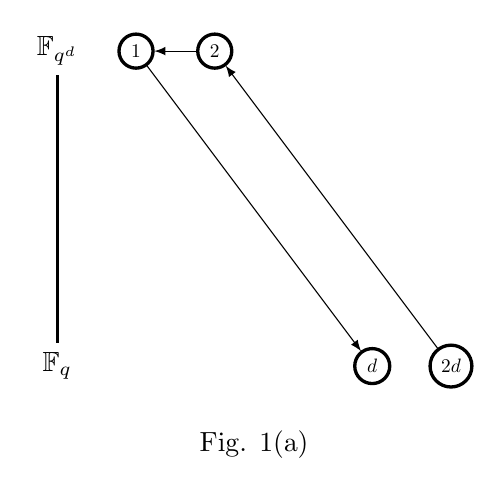
\begin{tikzpicture}
  \node (A) at (0,0) {$\mathbb{F}_{q}$}; 
  \node (B) at (0,4) {$\mathbb{F}_{q^{d}}$}; 
  \draw[very thick] (A) -- (B);

  \node[round] (2d) at (5, 0) {$2d$};
  \node[round] (2) at (2, 4) {$2$};
  \node[round] (1) at (1, 4) {$1$};
  \node[round] (d) at (4, 0) {$d$};

  \draw[arrow] (2d) -- (2);
  \draw[arrow] (2) -- (1);
  \draw[arrow] (1) -- (d);

  \node (t) at (2.5, -1) {Fig. 1(a)};
  
\end{tikzpicture}
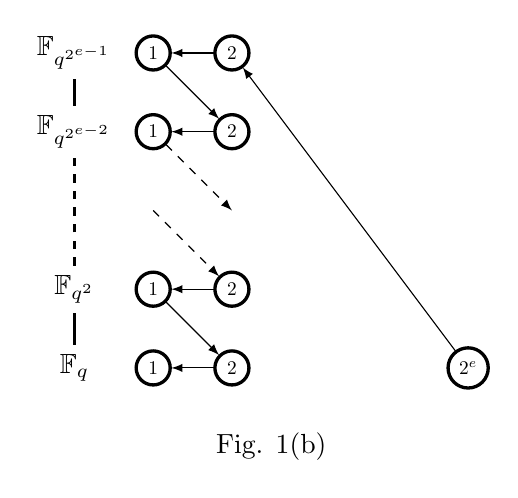
\begin{tikzpicture}
  \node (A) at (0,0) {$\mathbb{F}_{q}$};
  \node (B) at (0,1) {$\mathbb{F}_{q^2}$};
  \node (C) at (0,3) {$\mathbb{F}_{q^{2^{e-2}}}$};
  \node (D) at (0,4) {$\mathbb{F}_{q^{2^{e-1}}}$};

  \draw[very thick] (A) -- (B);
  \draw[very thick] (C) -- (D);
  \draw[dashed, very thick] (B) -- (C);

  \node[round] (1d) at (1, 4) {$1$}; 
  \node[round] (2d) at (2, 4) {$2$}; 
  \node[round] (1c) at (1, 3) {$1$}; 
  \node[round] (2c) at (2, 3) {$2$}; 
  \node[round] (1b) at (1, 1) {$1$}; 
  \node[round] (2b) at (2, 1) {$2$}; 
  \node[round] (1a) at (1, 0) {$1$}; 
  \node[round] (2a) at (2, 0) {$2$}; 
  \node[round] (E) at (5, 0) {$2^e$};

  \draw[arrow] (E) -- (2d);
  \draw[arrow] (2d) -- (1d);
  \draw[arrow] (1d) -- (2c);
  \draw[arrow] (2c) -- (1c);
  \draw[arrow] (2b) -- (1b);
  \draw[arrow] (1b) -- (2a);
  \draw[arrow] (2a) -- (1a);

  \draw[dashed-arrow] (1c) -- (2, 2);
  \draw[dashed-arrow] (1, 2) -- (2b);

  \node (t) at (2.5, -1) {Fig. 1(b)};
\end{tikzpicture}
  \caption{Two different possible strategies to perform the descent, the arrows
  $\nwarrow$, $\leftarrow$, and $\searrow$ stands respectively for
factorization and embedding in a larger field, on-the-fly degree $2$
elimination, and taking a norm and projecting in a subfield. The numbers
represent the degrees of the involved elements.}
  \label{fig:recurse}
\end{figure}

The discussion about the complexity is very similar to the one we had for the
BGJT algorithm. Performing the
descent, a tree is built in which the logarithm of a node is expressed
as a linear combination of its children. The total complexity of the algorithm
is then the number of nodes of this tree. We have seen that the arity of the
tree is $q+2$, and the height of the tree is $O(\log n)$, the number of nodes
is then $(q+2)^{\log n}$. Since we are in the small characteristic case, we
can write this complexity $l^{O(\log l)}$, where $l=\log(q^n)$ is the bitsize of
$\mathcal G$, and we see that the algorithm is quasi-polynomial.

\subsection{Some concluding remarks}

Similarly to the BGJT algorithm case, there are polynomials that cannot be
descended using the on-the-fly elimination. Once again, it happens when
dealing with a polynomial dividing the equation that defines our field.
Nevertheless, these polynomials can be dealt with and details can be found
in~\cite{GKZ14}. Two heuristics remain in this algorithm:

\begin{itemize}
  \item The existence of suitable polynomials $h_0$ and $h_1$, in order to be
    able to perform the on-the-fly elimination.
  \item The existence of a polynomial time algorithm to compute the logarithm
    of the elements of degree up to $4$. Indeed, we recall the the polynomial
    time algorithm of Propositon~\ref{prop:bgjt}, \ie the building block of
    BGJT algorithm, is heuristic.
\end{itemize}

In practical works, summarised in Gora Adj's PhD thesis~\cite{Adj16}, we
    can see that this algorithm is not really used all the way from elements
    of high degree (\ie $\geq 200$ in~\cite{Adj16}) to elements in the factor base. Instead, other descents  are first used to reduce the degree of the elements
    until having elements of small degree (\ie $\leq 16$ in~\cite{Adj16}).
    Furthermore, even when using the powers-of-2 algorithm, it is mixed with
    Joux's $L(1/4)$ algorithm, in order to deal with the element of odd
    degree. If this mixed algorithm was not used with elements of higher
    degree, it is probably because the on-the-fly elimination was using
    Gröbner bases algorithms, that have an exponential complexity. Hence, even
    if really efficient with elements of small degree, the cost is definitely
    too high with elements of large degree. We could try to use root
    finding instead of Gröbner bases, in order to obtain a polynomial
    complexity, and start to use the on-the-fly elimination earlier. But as we
    are going to see in Section~\ref{sec:results}, the root finding is probably
    too low to use this idea.
% Je ne suis pas sûr que ce blabla sur la pratique soit à la bonne place.

    
\section{Experimental results}
\label{sec:results}

All the material discussed in this section is available at
\url{https://github.com/erou/DlogGF.jl}. It is published as a
Julia~\cite{Julia} package, depending on the Nemo package~\cite{Nemo}. We first give
a very brief introduction to Julia and Nemo.
\subsection{Julia and Nemo}
\paragraph{Julia.} Julia is a free and open-source, high-level
programming language developed
since 2012, with dynamic type system and high-performance. It is a compiled
language, with a just-in-time (jit) compilation, meaning that the compilation
is almost invisible for the user but performances are comparable with
other compiled languages. It is easy to learn and to read,
especially for someone who already worked with a high-level language like
Python. There are many other interesting things to say about this new
language, the interested reader can find additional informations on Julia's
website and, of course, in the documentation of the language. Julia is designed for numerical computing, but there are some
symbolic computer algebra packages, such as Nemo.

\paragraph{Nemo.} Nemo is a computer algebra package for Julia. It aims to cover
commutative algebra, number theory and group theory. It contains wrappers for
MPIR, Flint, Arb and Antic, and other features written in Julia. 

\paragraph{Why Julia/Nemo ?}

One of the advantages of Julia is that it is fairly easy to directly call C
functions contained in other libraries. Therefore, all the Nemo functions
that we used in \texttt{DlogGF.jl} were in fact Flint functions. This
provides efficiency, the main reason why we use the duo Julia/Nemo, as well as
simplicity, because we are not directly using the C programming
language. On top of that, if a Flint function is not available in Nemo, we
can directly call it from Julia.

\subsection{The BGJT algorithm}

We recall that for Heuristic~\ref{heur:full-rank} to hold, we must have that $q$
is not too small, because the expected number of equations is $\Theta(q^3)$,
and the number of unknowns is $q^2+1$ or $q^2$. When we compute the factor
base, our unknowns are the $\log(X + a)$, for
$a\in\mathbb{F}_{q^2}$, and $h_1$. In our experiments, the heuristic holds as
soon as $q\geq 7$, but not for every choice of parameters $h_0$ and $h_1$. When
$q\geq 11$, it holds in every experiment. In the descent part, the constant hidden in the
$\Theta(q^3)$ depends on the degree of the target element, but it is definitely
smaller than when working with linear elements. Therefore the integers $q$
for which the heuristic holds are larger.

We give timing results for the computation of the factor base, \ie the linear
elements and $h_1$, in fields of the form $\mathbb{F}_{q^{2q}}$. Since elements are
represented as polynomials with coefficients in $\mathbb{F}_{q^2}$, there are
$q^2+1$ elements in the factor base.
\begin{center}
\begin{tabular}[here]{cccc}
  Field & Bitsize & Timing (seconds) & Linear algebra \\
  $\mathbb{F}_{7^{14}}$ & $39$ & $0.20$ & $5$\% \\
  $\mathbb{F}_{11^{22}}$ & $76$ & $1.5$ & $23$\% \\
  $\mathbb{F}_{17^{34}}$ & $139$ & $16$ & $59$\% \\
  $\mathbb{F}_{23^{46}}$ & $208$ & $140$ & $79$\% \\
  $\mathbb{F}_{29^{58}}$ & $282$ & $990$ & $79$\% \\
\end{tabular}
\end{center}
We see that the linear algebra is the main operation. For example, in the last
computation (in $\mathbb{F}_{29^{58}})$, the other main steps were finding the
factors of the order of the group, \ie factoring $29^{58}-1$, ($10$\% of the
time), computing the logarithms modulo the small factors with the Pohlig-Hellman
algorithm ($5$\% of the time), the other $6$\% being various polynomial
manipulations, such as determining if a polynomial is smooth. The linear
algebra step uses standard Gaussian elimination modulo each large factor of the
cardinal of the group, performed on a matrix of size
$\Theta(q^3)\times(q^2+1)$, for an expected complexity of $O(q^6)$. In examples
of cryptographic size, for example with a bitsize of $4000$, the linear algebra
is known to be the bottleneck of the computations. Note that, since the matrix
is sparse, we can obtain a complexity of $O(q^5)$ using sparse linear algebra.
With some optimisations, and assuming that the factorization of the cardinal of
the group is given, the other manipulations should be negligible.

\subsection{The powers-of-2 algorithm}

\section*{Acknowledgements}

Of course, this work could not have been done without the help and advices of my
supervisors, and I am very grateful that they let me work on this very exciting
subject. I would also like to warmly thank Gora \textsc{Adj} for the
precious explanations he gave me during all the internship, his expertise on the
subject was helpful at the very least. Finally, I would like to thank all the
people in the SCG lab for their welcome, and for the times chatting, having
lunch, or \href{http://www.keeptalkinggame.com/}{defusing bombs}.

\bibliographystyle{plain}
\bibliography{dlog}
\end{document}
